%!TeX root=MemoriaTFG.tex

\chapter{System analysis and design}\label{chap:design}

\section{Users and operating context}

Wave Launcher is designed for a player who owns Minecraft: Java Edition and wants to host a private server from a Windows computer. The target user can select gameplay options, Minecraft versions or mods, but is not assumed to understand Java compatibility, command-line flags, directory layouts, dependency graphs or network address translation. This distinction determines where responsibility lies. The user decides what kind of server is wanted; the program converts that intent into files, processes and provider requests.

The application is local and single-user. It is not an administration service intended to remain active independently of its interface, and it does not provide accounts or remote multi-user control. A server process exists only while Wave Launcher is running. This behavior gives the user a simple mental model: closing the program also ends the locally managed sessions. Persistent configuration survives between launches, but execution state does not.

The main workflows are server creation, edition of an existing server, execution and console interaction, Java management, and application configuration. Mod management is part of server revision rather than a separate global library because compatibility depends on the selected Minecraft version and mod loader.

\begin{figure}[htbp]
  \centering
  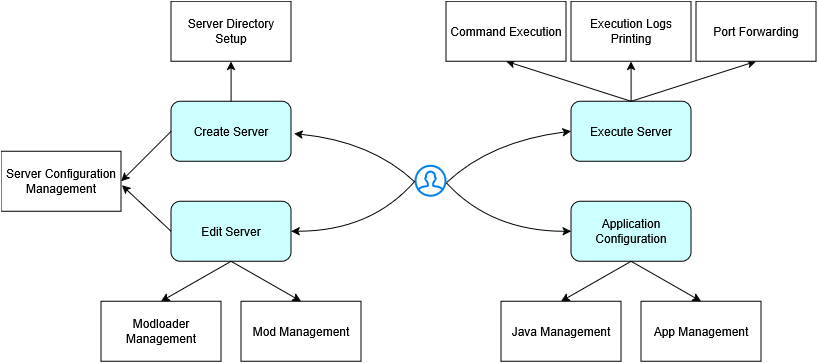
\includegraphics[width=\textwidth,height=0.72\textheight,keepaspectratio]{User Workflows.png}
  \caption{Principal user workflows in Wave Launcher.}
  \label{fig:workflows}
\end{figure}

\section{Quality requirements}

The functional requirements in Section~\ref{sec:scope} state what the application must do. Several non-functional properties constrain how those operations are implemented.

\paragraph{Usability.} Server management must be possible without editing a JSON file, a properties file or a command line. Technical failures must be converted into visible messages, and long operations must show that work is in progress. Related selections must be filtered so that the interface does not knowingly offer impossible combinations.

\paragraph{Compatibility.} The completed product targets Windows. Provider and domain components should not depend on Windows when their work is portable, allowing another platform adapter to be added later. Minecraft, loader, mod and Java compatibility must be derived from provider metadata rather than encoded as a fixed list wherever such metadata exists.

\paragraph{Maintainability.} External systems must be replaceable without rewriting the central use cases. File persistence, image conversion, server execution, Java acquisition, mod catalogues and port mapping are consequently accessed through application interfaces.

\paragraph{Recoverability.} Persistent metadata must remain readable across normal application restarts. Failed downloads should not be recorded as successful installations. Migration must report components that cannot be retained. Since the current application modifies a real server directory rather than a transactional store, complete rollback of every file operation is not guaranteed; this constraint is relevant when interpreting the migration design.

\paragraph{Responsiveness.} Network, installation and process operations use asynchronous interfaces so that the UI thread is not intentionally blocked while files are obtained or a catalogue is queried. The interface displays a busy overlay during operations that cannot complete immediately.

\paragraph{Security and privacy.} Server worlds, configuration and Java runtimes remain on the local computer. CurseForge credentials are application configuration and must not be embedded in source code. Port mapping is requested only when a server is started and is released when it stops or startup fails.

\section{Architectural design}

\subsection{Choice of architectural style}

Wave Launcher follows a hexagonal architecture. At the centre are domain objects describing servers, Java installations, Minecraft versions, mod loaders, mods and device information. The application project surrounds this model with ports. Input ports express the operations available to the interface, while output ports describe what the application needs from files, remote providers and the operating system. The infrastructure project supplies the corresponding adapters and orchestration services.

This structure is useful because Wave Launcher depends on many replaceable external mechanisms. A Modrinth response and a CurseForge response have different schemas, but neither schema needs to leak into the server editor. Both adapters map their data into the same domain types. The same applies to Mojang and Adoptium Java packages, Forge and Fabric loaders, and JSON repositories. The design does not remove provider differences, such as the CurseForge token requirement, but it gives those differences a defined location.

Infrastructure contains both adapters and implementations of application services. The object graph is assembled manually by the \texttt{AppComposition} composition root instead of by a dependency-injection container. I evaluated dependency injection during development, but its integration with the MAUI interface made the creation of UI components disproportionately complex for this project. The extra indirection also made new screens harder to follow without giving a clear benefit at the current scale. Manual composition was therefore chosen as the simpler option. It produces a long initialization method, but every adapter, service and view-model dependency can be traced from one place. Section~\ref{sec:implementation-composition} shows how this decision appears in the code.

\begin{figure}[htbp]
  \centering
  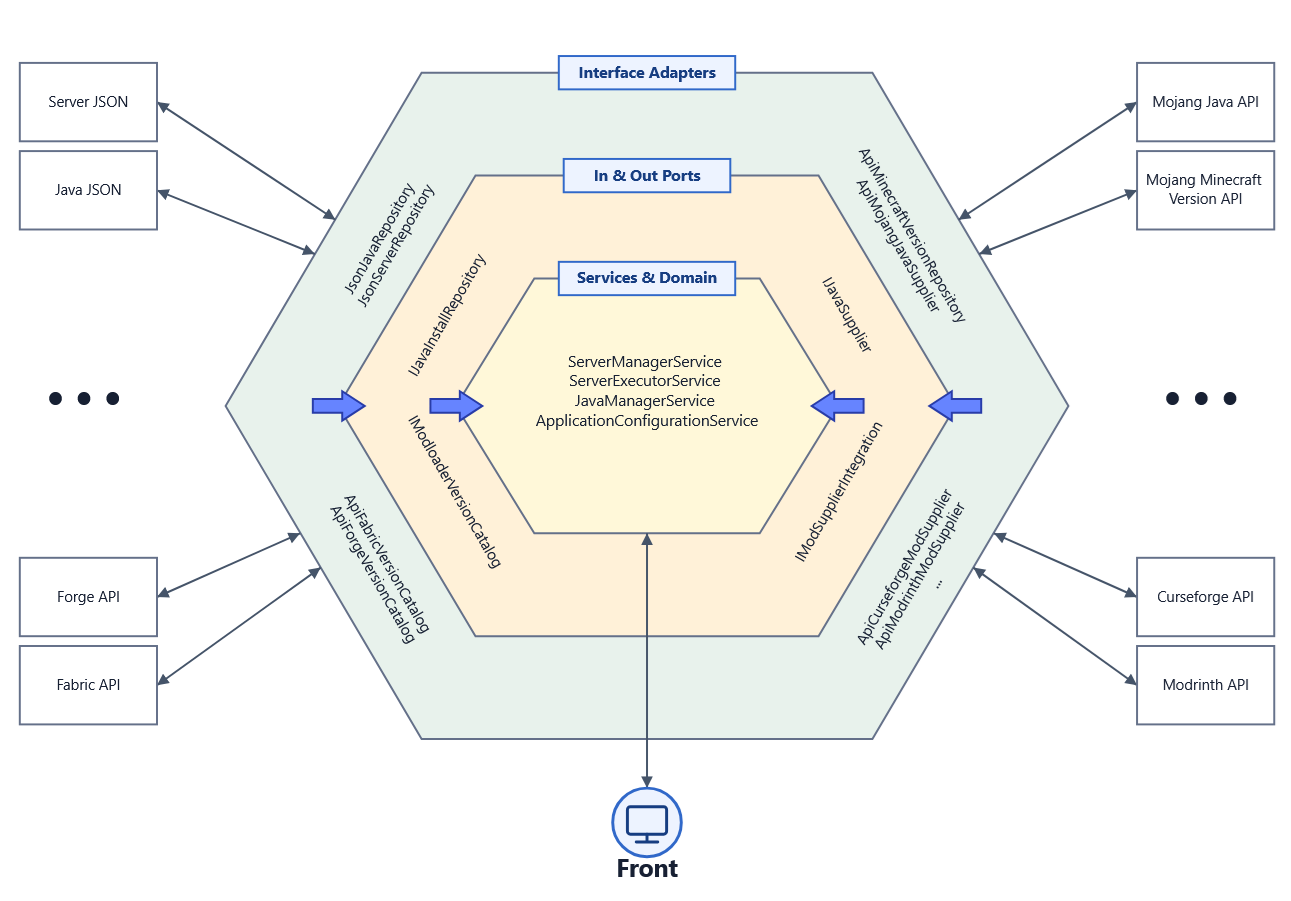
\includegraphics[width=\textwidth,height=0.72\textheight,keepaspectratio]{Hexagonal Architecture.png}
  \caption{Hexagonal architecture and dependency direction.}
  \label{fig:hexagonal}
\end{figure}

\subsection{Solution projects}

The solution is divided into four projects.

\begin{description}
  \item[Wave.Domain] contains records, entities, enumerations and state shared by the use cases. It has no reference to the interface or infrastructure projects.
  \item[Wave.Application] defines input, intermediate and output contracts. It references the domain because its operations exchange domain objects.
  \item[Wave.Infrastructure] implements repositories, external catalogues, installers, process execution, image transformation, port mapping and the services that coordinate them.
  \item[Wave.Ui] provides the .NET MAUI application, XAML pages, reusable controls and view models. It is also the composition root that connects concrete adapters to their interfaces.
\end{description}

Dependencies point inward toward the domain and application contracts. The domain does not know that persistence uses JSON or that the graphical layer uses MAUI. Infrastructure can be replaced one adapter at a time as long as the corresponding contract remains meaningful.

\section{Domain model}

\subsection{Server aggregate}

The \texttt{Server} class is the central persistent object. It has a generated identifier, a display name, optional icon data, execution flags, EULA state and a dictionary of server properties. It refers to a \texttt{MinecraftVersionInstallation}, an optional \texttt{ModloaderInstallation}, a collection of \texttt{ModFile} objects and a selected \texttt{JavaInstallation}. The model stores the state required to reopen the server editor without rediscovering every choice from the file system.

Runtime state is deliberately excluded from this aggregate. A running Java process is represented by \texttt{IServerSession} and held by \texttt{IServerExecutorService}. This prevents process handles and observable output streams from being serialized. It also makes a clear distinction between a \texttt{Server} definition, which is persistent, and a server session, which exists only in memory.

\texttt{ServerQuery} is used as an editable transfer model for creation and modification. It can contain catalogue-level choices such as \texttt{MinecraftVersionInfo} before they have become installed artifacts. Comparing a query with the stored server produces \texttt{ServerChanges}, which lets the interface show the consequences of modifying or updating a server.

\subsection{Version and installation types}

Catalogue information and installed information are separate types. A \texttt{MinecraftVersionInfo} catalogue item contains an identifier, type and details URL. Retrieving \texttt{MinecraftVersionDetails} supplies the server download and required Java version. Once installed, the server holds a \texttt{MinecraftVersionInstallation}. A similar distinction exists among \texttt{JavaVersion}, \texttt{JavaPackage} and \texttt{JavaInstallation}, and among \texttt{ModloaderInfo}, \texttt{ModloaderPackage} and \texttt{ModloaderInstallation}.

This separation prevents a remote URL from being mistaken for a local artifact. It is particularly important for Java, where a supplier can expose compressed archives or a manifest made of many files. The installer chosen for a package creates a normalized \texttt{JavaInstallation} with an executable path that server execution can consume without knowing how the runtime was delivered.

\subsection{Mod representation}

Mods require more metadata than a simple file path. \texttt{ModInfo} identifies a project and its supplier; \texttt{ModVersion} describes a compatible release; and \texttt{ModFile} combines project and version information for installation. A mod file contains artifacts and dependencies. Dependencies are classified so that required and incompatible relations can influence installation.

Supplier identity remains in the domain model through \texttt{ModSupplierType} because identifiers from Modrinth and CurseForge are not interchangeable. This is an intentional provider distinction, unlike the HTTP response types, which remain inside their adapters. \texttt{PaginationState} is also represented independently so the same UI component can browse catalogues without depending on one provider's pagination fields.

\section{Ports and adapters}

\subsection{Input ports}

Input ports group operations by user intention. \texttt{IServerManagerService} creates, edits, deletes and retrieves server definitions. \texttt{IServerExecutorService} starts and stops sessions and submits commands. \texttt{IMinecraftCatalogService}, \texttt{IModloaderCatalogService} and \texttt{IModCatalogService} retrieve Minecraft versions, mod loaders and mods respectively. \texttt{IJavaManagerService} lists suppliers and installations and performs installation or removal. Application configuration and device information are exposed through \texttt{IApplicationConfigurationService} and \texttt{IDeviceInformationService}.

Separating management from execution avoids making the server entity responsible for process control. It also lets the servers page query execution state independently of the saved configuration. The interface works through these contracts, which keeps view models from reading JSON files or starting \texttt{java.exe} directly.

\subsection{Intermediate services}

Some operations are meaningful only as part of server management but still deserve isolated responsibilities. \texttt{IVersionManagerService} downloads the selected Minecraft server artifact. \texttt{IPropertiesManagerService} and \texttt{IEulaManagerService} translate domain state to the text files consumed by Minecraft. \texttt{IModloaderManagerService} and \texttt{IModManagerService} install and migrate their respective components. \texttt{IServerPathResolver} gives all of these services a consistent directory layout.

Together, these services make it possible to treat creation and editing as coordinated workflows rather than as unrelated file operations. Creation has to respect the dependencies between the server directory, Minecraft version, native configuration files, optional loader, mods and persisted metadata. Editing first identifies what changed and then invokes the managers affected by that change. The exact order and the corresponding service calls are discussed in the implementation chapter.

\subsection{Output ports}

Output ports cover persistence, providers and operating-system facilities. \texttt{IServerRepository}, \texttt{IJavaInstallRepository} and \texttt{IApplicationConfigurationRepository} store servers, Java installations and application configuration. \texttt{IMinecraftVersionRepository} and \texttt{IModloaderVersionCatalog} obtain Minecraft and loader versions. \texttt{IModSupplierIntegration} and \texttt{IJavaSupplier} represent remote mod and Java providers. \texttt{IServerExecutor} executes servers, \texttt{IImageTransformer} transforms images, \texttt{IDeviceInformationRepository} reads device information, and \texttt{IPortMapper} creates network mappings.

Each adapter owns the translation between an external representation and the domain. \texttt{ApiMinecraftVersionRepository} deserializes Mojang's version manifest and maps its DTOs to version information. \texttt{ApiForgeVersionCatalog} parses Forge's Maven metadata as XML. Fabric, Modrinth, CurseForge and Adoptium responses use provider-specific DTOs within their respective adapters. \texttt{JsonServerRepository}, \texttt{JsonJavaRepository} and \texttt{JsonApplicationConfigurationRepository} serialize persistent domain state, while \texttt{WindowsServerExecutor} wraps \texttt{System.Diagnostics.Process}.

\section{Persistence and directory design}

JSON persistence was chosen because the data volume and relationships are small. The application needs to retain application settings, the list of managed Java installations and the configuration of each server. A relational database would add deployment and mapping complexity without providing a material benefit for the current access patterns. Server worlds and executable artifacts already live as files, so the JSON documents are metadata rather than the only copy of the installation.

Repository interfaces keep that decision reversible. If later versions need concurrent access, querying over many users or stronger transactions, a database adapter can implement the same repository roles. Some contract changes might still be needed for efficient querying, but UI and provider code would not have to know the storage technology.

\texttt{ServerPathResolver} centralizes the application directory, server collection, Java collection and temporary workspace. Each \texttt{Server} receives its own root directory. Files such as \texttt{server.properties}, \texttt{eula.txt}, the vanilla server JAR, the normalized loader JAR and the \texttt{mods} directory are derived from that root. Central path construction reduces the risk that different managers disagree about where an artifact belongs.

\begin{figure}[htbp]
  \centering
  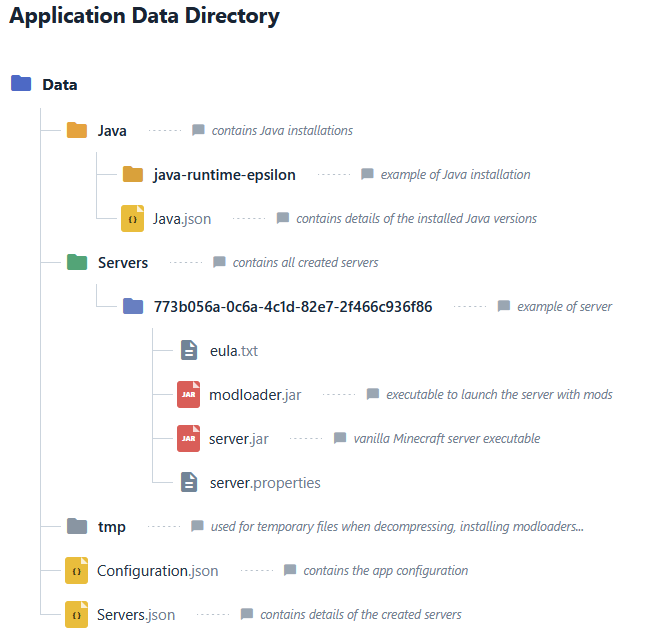
\includegraphics[width=\textwidth,height=0.72\textheight,keepaspectratio]{Application Directory.png}
  \caption{Application data and server directory layout.}
  \label{fig:directories}
\end{figure}

\section{Design of the principal workflows}

This section describes the responsibility and order of each workflow. It intentionally stays at design level. Concrete methods, control flow and selected code excerpts are presented in Chapter~\ref{chap:implementation}.

\subsection{Server creation and editing}

The server editor collects the chosen Minecraft release, Java runtime, properties, icon, execution flags and EULA value in an editable query. Required information is validated before the query reaches the application service. The creation workflow then constructs a persistent server definition and performs the necessary file operations in dependency order.

Editing uses the same conceptual form but begins from the stored aggregate. At this stage, the mod-loader and mod-management controls become available because the initial server setup has already been completed and the application has a concrete Minecraft version and directory against which compatibility and installation operations can be performed. \texttt{ServerManagerService} compares installed state with the submitted \texttt{ServerQuery} and coordinates both the requested edit and any additional changes needed to preserve compatibility. A Minecraft version change downloads the new server software and reevaluates the installed loader and mods against the selected release. Changing the mod-loader type also causes the mod set to be reevaluated because mods built for one loader cannot be retained under another without a compatible replacement. Even when the Minecraft version and loader remain unchanged, adding or replacing a mod can produce further changes: \texttt{ModManagerService} follows its required dependencies, adds compatible dependency files automatically and rejects declared incompatibilities.

The edit workflow returns its automatic consequences as a change summary. This summary identifies a loader that had to be removed and separates mods into deleted, failed, incompatible and automatically required collections. When no additional compatibility action is needed, there is no summary to display. Otherwise, the interface uses it to explain why the final installation may differ from the choices made directly by the user. The resulting metadata is saved only after the management workflow has applied both the requested and automatic changes.

The design favors a single coherent edit over a set of isolated buttons that can silently produce incompatible state. The change-summary popup makes potentially destructive consequences visible before confirmation.

\begin{figure}[htbp]
  \centering
  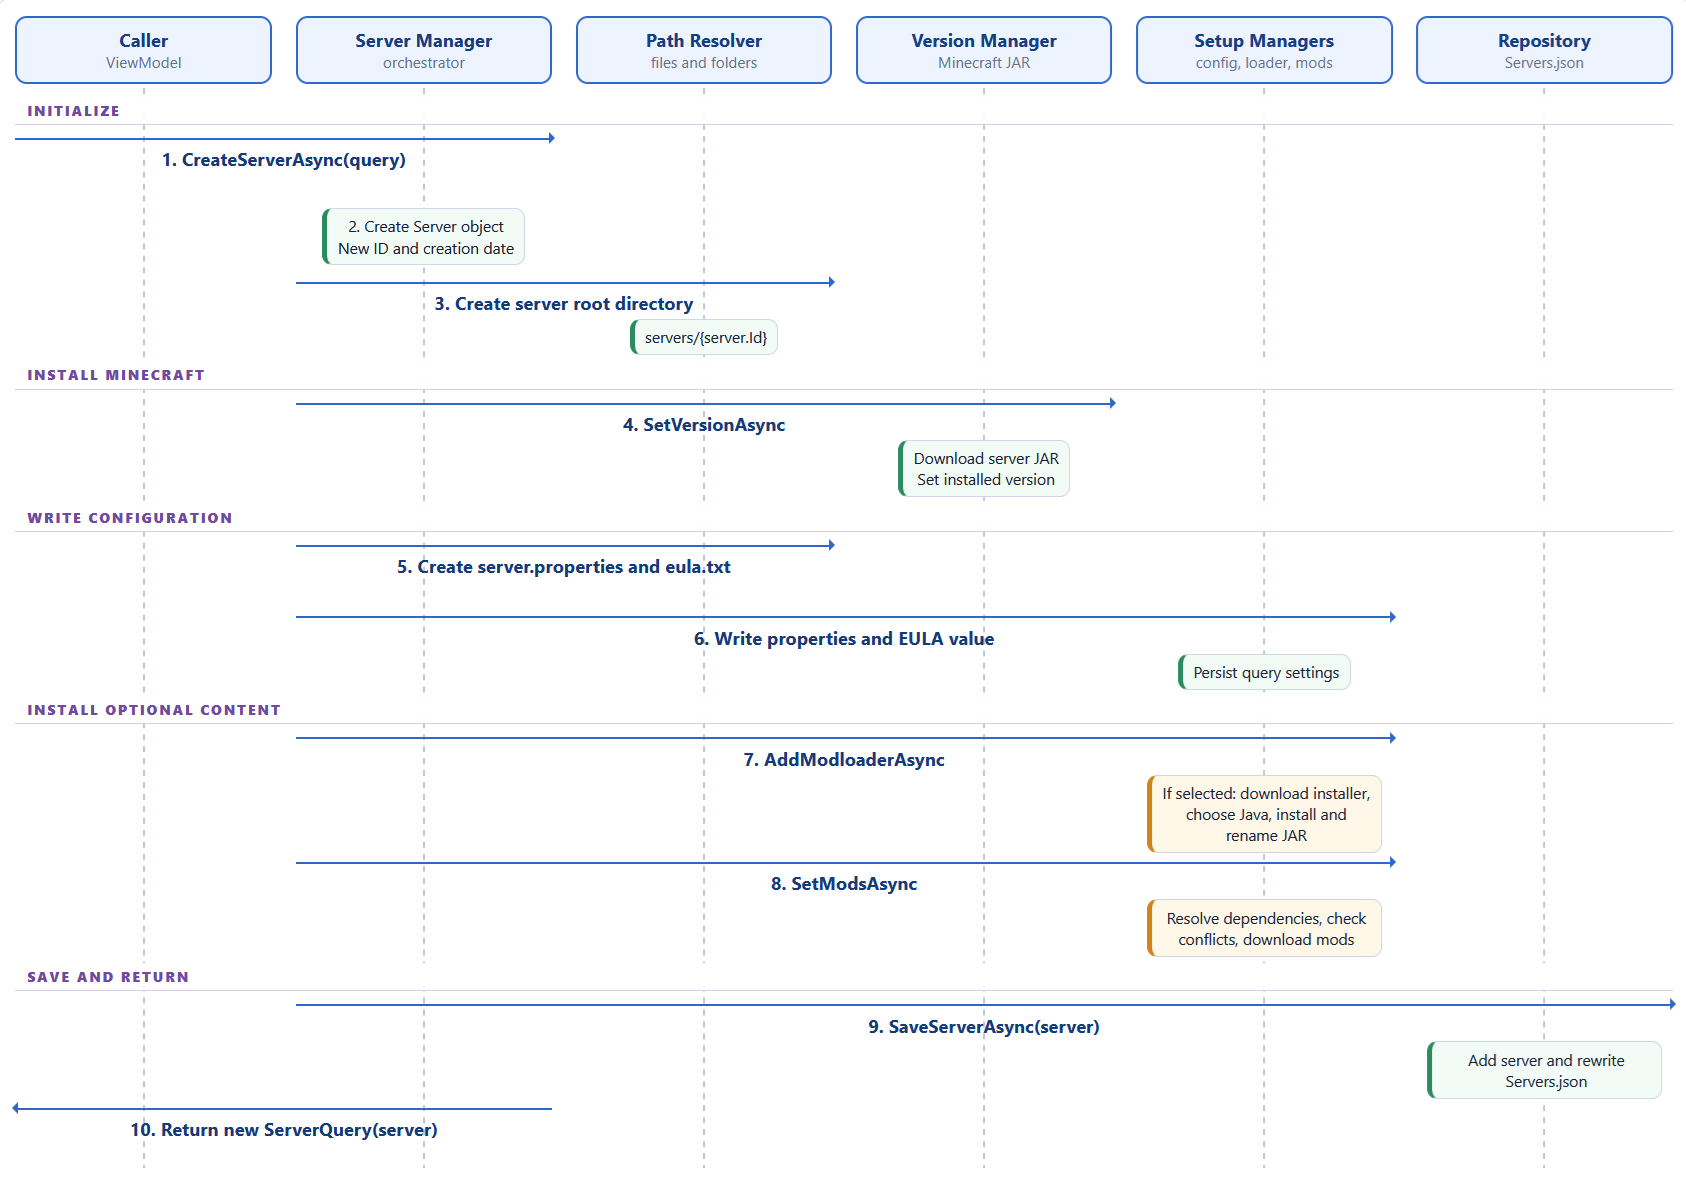
\includegraphics[width=\textwidth,height=0.72\textheight,keepaspectratio]{Server CreationSequence.png}
  \caption{Sequence for creating a server instance.}
  \label{fig:create-sequence}
\end{figure}

\subsection{Java management}

Java management starts from the device operating system and architecture, which restrict the supplier results to usable packages. The two supported suppliers use different delivery formats: Adoptium provides compressed releases, whereas Mojang provides runtime manifests. The design represents both as Java packages, chooses an installer according to the package type and normalizes the result as a managed Java installation.

Only managed installations are presented as Wave installations. This avoids changing a system-wide Java configuration and lets multiple major Java versions coexist. A runtime cannot be removed when a saved server depends on it. During server execution, the selected installation supplies the exact executable path rather than relying on the system \texttt{PATH}.

\subsection{Mod-loader management}

The mod-loader workflow selects a catalogue according to the requested loader type. Forge derives its versions from Maven metadata, while Fabric exposes public catalogue endpoints. Despite this difference, both produce the same domain-level package and installation concepts. Packages are downloaded to temporary storage, installed with a managed Java runtime and normalized to a predictable loader path.

A server can have at most one loader. Changing the Minecraft version asks the catalogue for a loader release compatible with the new game version. If none exists, the loader is removed and the result is reflected in the server state. Removing a loader also removes associated mods because they cannot be assumed to run without that environment.

\subsection{Mod discovery and dependency resolution}

\texttt{ModsPopupViewModel} sends the selected Minecraft version, loader and \texttt{PaginationState} to an \texttt{IModSupplierIntegration}. Results are therefore constrained before the user chooses a release. \texttt{ApiCurseforgeModSupplier} requires a token supplied through application settings; \texttt{ApiModrinthModSupplier} does not require the same credential.

When mods are added, \texttt{ModManagerService} recursively resolves required dependencies. A visiting set prevents cycles from causing unbounded recursion. Already installed or already planned projects are not downloaded twice. Incompatible relationships are checked in both directions because either the candidate or an installed mod can declare the conflict. Automatically added dependencies are returned in \texttt{ModMigrationResult} so that the interface can explain the final set.

Migration reevaluates every mod whose Minecraft version or loader differs from the changed server. The old artifact is removed, the supplier is asked for compatible releases and the newest returned version is selected. The result distinguishes deleted, failed, incompatible and automatically required mods. This information is more useful than a single success flag because a valid server migration can still mean that a particular mod is no longer available.

\begin{figure}[htbp]
  \centering
  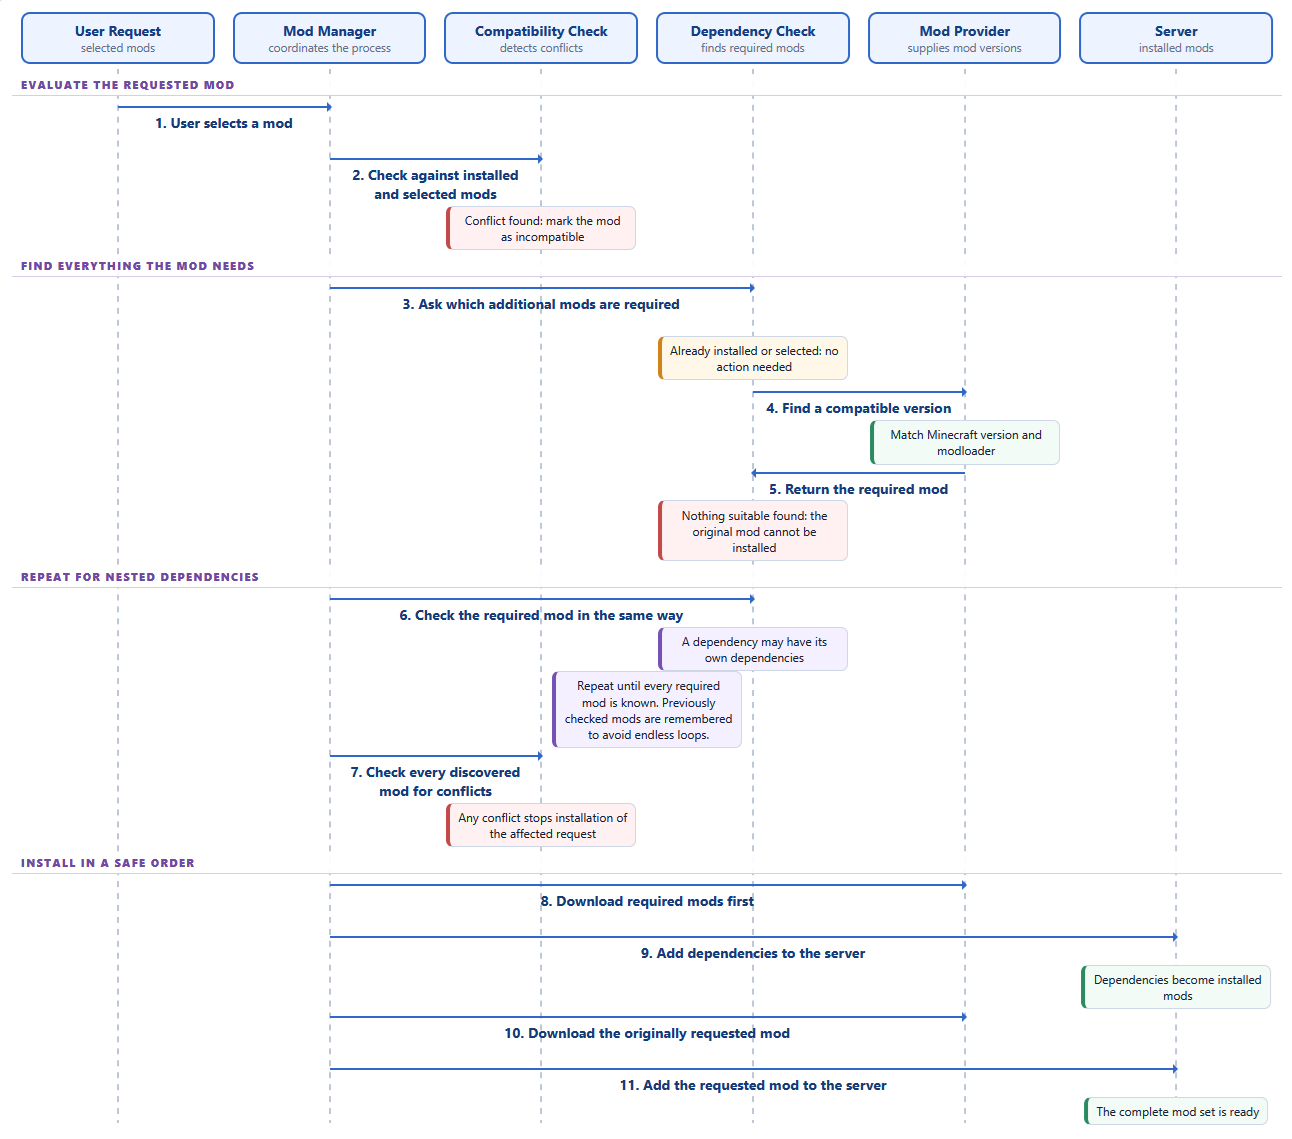
\includegraphics[width=\textwidth,height=0.72\textheight,keepaspectratio]{RecursiveModResolution.png}
  \caption{Recursive resolution of required and incompatible mods.}
  \label{fig:dependencies}
\end{figure}

\subsection{Execution and port mapping}

Starting a server is a coordinated local and network operation. \texttt{ServerExecutorService} first rejects a second start of the same instance and checks whether another Wave session uses the requested port. It then requests a temporary mapping through \texttt{IPortMapper}. \texttt{SharpOpenNatPortMapper} attempts UPnP and NAT-PMP discovery and creates a TCP mapping with the same private and public port. If discovery or mapping fails, startup returns a specific \texttt{ServerStartResult} and the Java process is not launched.

After mapping succeeds, \texttt{ServerExecutorService} chooses the server or loader JAR, obtains the configured Java executable and asks \texttt{IServerExecutor} to start the process. Standard input, standard output and standard error are redirected through \texttt{IServerSession}. Output is exposed as an asynchronous sequence so \texttt{ExecutionViewModel} can append lines as they arrive. Commands written by the user go to standard input through \texttt{IServerSession.SendCommandAsync}.

The mapping is represented by \texttt{PortMappingLease} and owned by the private \texttt{RunningServer} record in \texttt{ServerExecutorService}. It is disposed when the server stops, when the process exits, or when process startup fails. This ownership is important because a mapping should not remain after the corresponding listener has gone away. Router support is still an environmental requirement: automatic mapping depends on UPnP or NAT-PMP being enabled and available.

\begin{figure}[htbp]
  \centering
  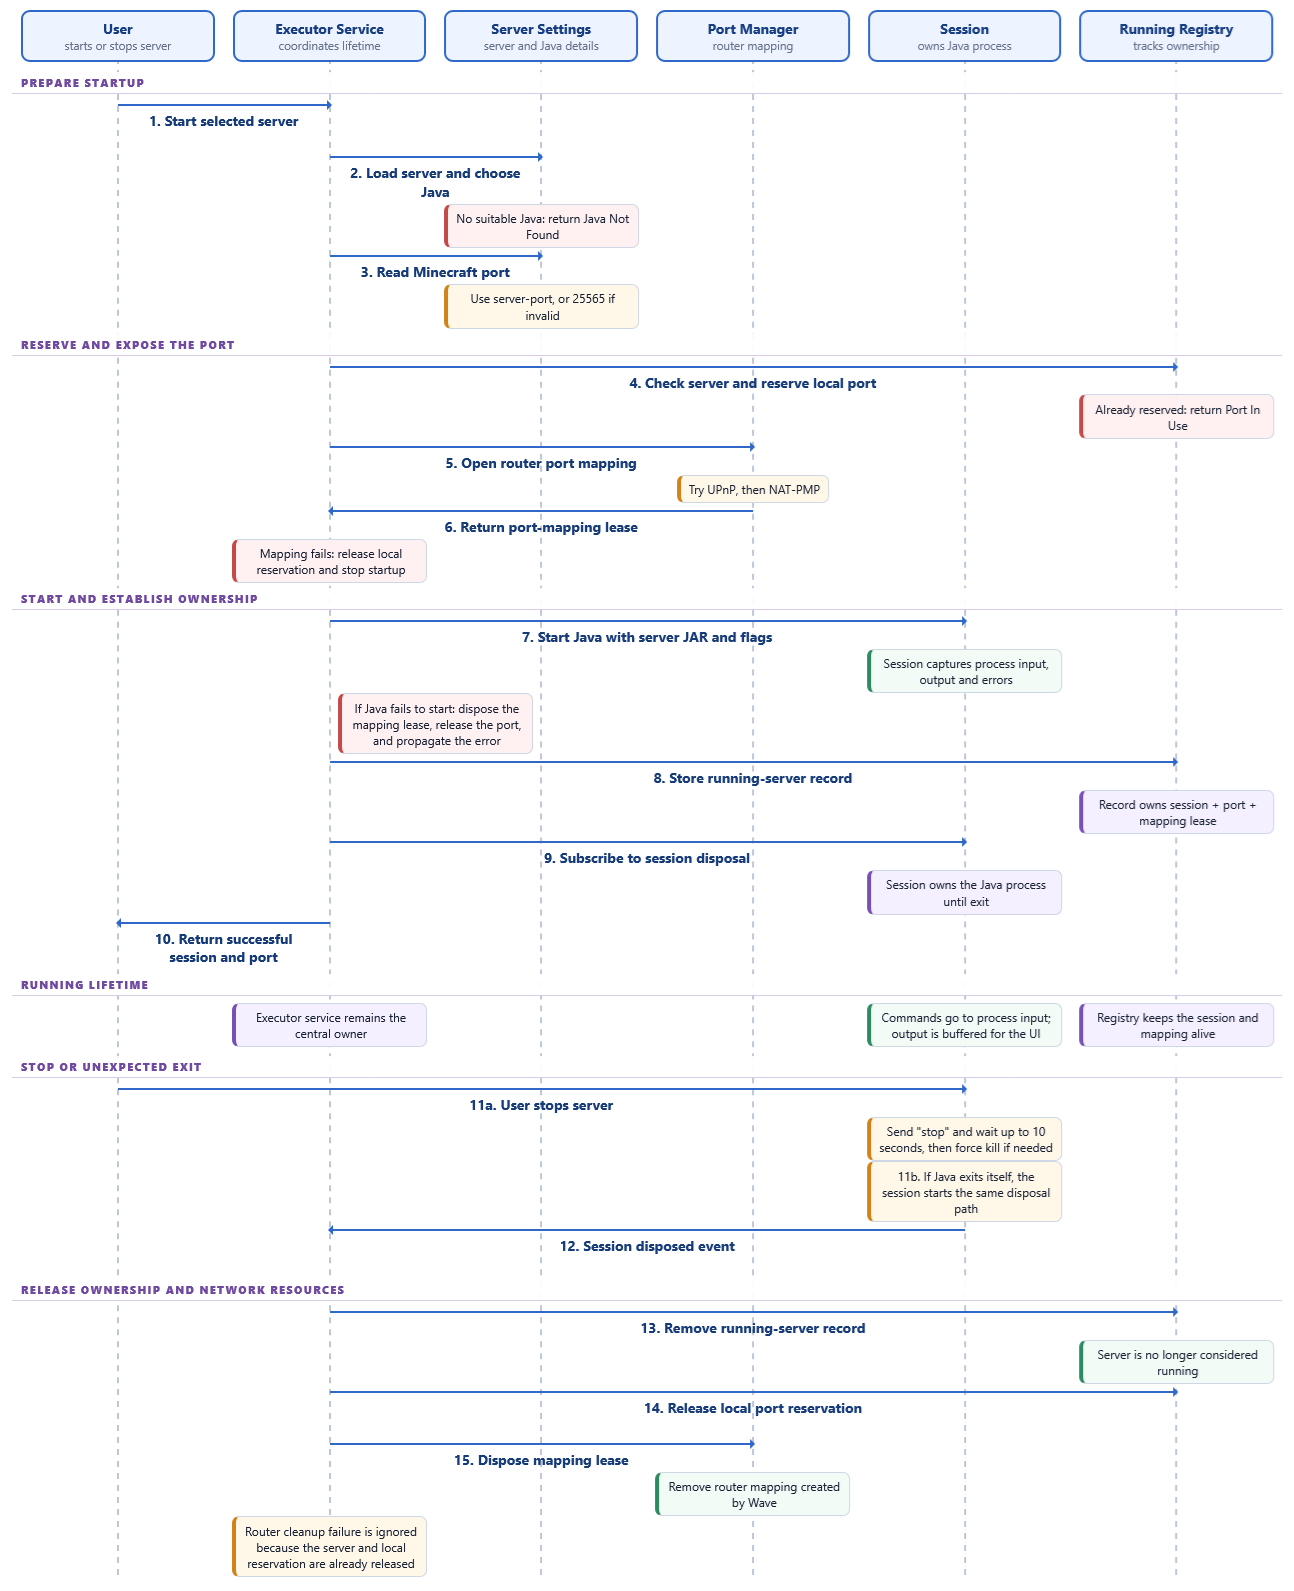
\includegraphics[width=\textwidth,height=0.72\textheight,keepaspectratio]{ServerExecution.png}
  \caption{Server startup, process ownership and port-mapping lifetime.}
  \label{fig:execution-sequence}
\end{figure}

\section{User-interface design}

The \texttt{Wave.Ui} project forms the presentation layer. It organizes the interface using XAML views and view-model classes: views define the visual structure, while view models expose screen state and invoke the application input ports. The project also contains \texttt{AppComposition}, which assembles the concrete infrastructure adapters and application services before supplying them to the view models. This keeps construction at the outer edge of the system and prevents the presentation components from instantiating repositories, provider clients or process executors themselves.

The application shell exposes three main destinations: servers, execution and settings. The servers page is the starting point and displays persistent instances as cards. Creating or selecting a card opens the server editor. The editor divides a large configuration into general, properties and mods views. The execution page concentrates transient process interaction, while settings contains Java and provider configuration.

View models use commands and observable properties from CommunityToolkit.Mvvm. The XAML views bind to those properties and do not call repositories or external providers. Custom form components standardize labels, validation and submission. A paginated collection component is reused for provider results, and a busy overlay prevents repeated submissions during long operations.

The visual design uses a dark palette and card-based grouping familiar to game launchers. Provider logos help distinguish Mojang, Adoptium, Forge and Fabric choices. Destructive actions are separated from ordinary editing, and a changes popup is used when an update may remove or replace dependent components.

\begin{figure}[htbp]
  \centering
  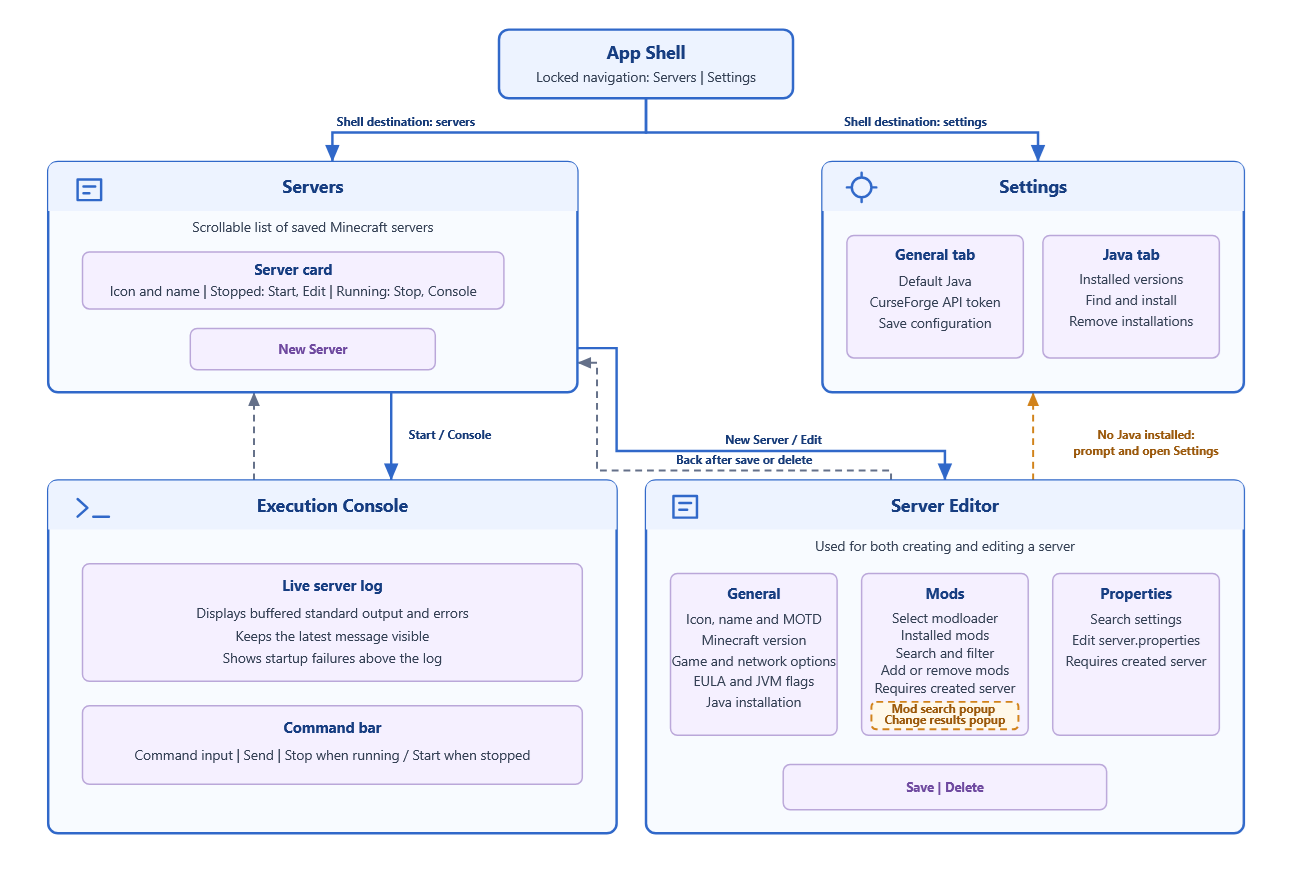
\includegraphics[width=\textwidth,height=0.72\textheight,keepaspectratio]{NavigationStructure.png}
  \caption{Navigation structure and principal application screens.}
  \label{fig:navigation}
\end{figure}

\section{Technology selection}

\subsection{C\#, .NET and MAUI}

C\# and .NET were selected both as a learning objective and for their suitability for a desktop application that performs HTTP, file-system and process operations. Asynchronous tasks, JSON serialization, process APIs and a mature package ecosystem cover the core technical needs without introducing a second server-side runtime.

.NET MAUI supplies a shared XAML and C\# UI project for Windows, Android, iOS and macOS. The present release is Windows-only because its executor and device-information adapters are Windows-specific and the project was validated on that platform. The framework choice nevertheless prevents the complete interface from being tied to a Windows-only widget toolkit. Supporting another desktop platform would require platform adapters and testing rather than a new application core.

A local web interface was the main alternative considered. It would have made browser technology available, but it creates a less direct lifecycle for the target user: launching an executable that opens a browser tab does not clearly communicate whether the underlying local service is still running. A desktop window provides an immediate indication that Wave Launcher and its server sessions are active. For a casual user installing a local tool, this model is closer to the expected behavior of an application.

\subsection{Libraries}

CommunityToolkit.Mvvm supplies observable properties and commands, while CommunityToolkit.Maui provides additional interface support. \texttt{System.Reactive} is used for process output. ImageSharp normalizes selected server icons. Markdig converts provider descriptions written in Markdown. SharpOpenNat provides UPnP and NAT-PMP discovery and mapping. HTTP clients and XML or JSON serializers implement provider communication.

These libraries are used behind project-level abstractions where their behavior affects the application core. SharpOpenNat, for example, is hidden by \texttt{IPortMapper}, and ImageSharp by \texttt{IImageTransformer}. UI-oriented libraries remain in the MAUI project because replacing the UI framework would already require new views and view models.

\subsection{Development environment}

Development was performed in Visual Studio Code with C\# Dev Kit, .NET MAUI tooling and NuGet Gallery. Todo Tree supported daily tracking. Git and GitHub supplied local history and remote backup, with major milestones used as commit boundaries. Hoppscotch assisted during the external API phase. Artificial-intelligence tools were used mainly while diagnosing programming defects. No diagramming application formed part of the development process; the architectural illustrations in this report document the resulting system rather than reproducing design artifacts created earlier.

\section{Design limitations}

The architecture reduces coupling but does not make external services reliable. Catalogue operations require internet access, CurseForge requires a user-provided API token, and automatic network exposure requires a compatible router configuration. The application must report these conditions but cannot remove them.

Persistence is simple and appropriate to a local single-user application, but JSON files and server directories do not provide a shared transaction. A failure at an unfortunate point in a multi-file migration may require recovery work beyond restoring one serialized object. Backups and staged directory replacement would strengthen a later release.
